\section{Module 70 : Static Single Assignment IR}
Consider the following example

    \[x = y+z\]
    \[x = x+1\]
    \[w=y+z\]
    \[z=x+3\]
    
In this example, the computation $y+z$ could be reused.
In SSA, we assign versions to variables(as below) and each version has only one assignment to it. SSA stands for single assignment in a static program. 
    \[x_1 = y+z\]
    \[x_2 = x_1+1\]
    \[w_1=y+z\]
    \[v_1=x_2+3\]
    
Using SSA, we can not optimize the code by rewriting $w_1 = y+z$ as $w_1 = x_1$.

    \[x_1 = y+z\]
    \[x_2 = x_1+1\]
    \[w_1=x_1\]
    \[v_1=x_2+3\]
    
Why SSA? Advantages of SSA:
\begin{itemize}
    \item Optimization algorithms become simpler if each variable has only one definition.
    \item Unrelated uses of same variable become independent.
    \item More values become available at each program point.
\end{itemize}
Therefore, SSA is a very popular method of IR design. LLVM IR is also an SSA IR.

\subsection{Converting to SSA}
\begin{itemize}
    \item Replace the target of each assignment with a new variable.
    \item Replace each use of a variable with the version of the variable reaching that point.
\end{itemize}
Again, taking an example:

    \[x = y+z\]
    \[a = b+x\]
    \[x=a+3\]
    \[y=x-a\]
On applying the two rules for conversion to SSA, these statements change to :
     \[x_1 = y+z\]
    \[a = b+x_1\]
    \[x_2=a+3\]
    \[y=x_2-a\]
    

\begin{figure*}
\centering
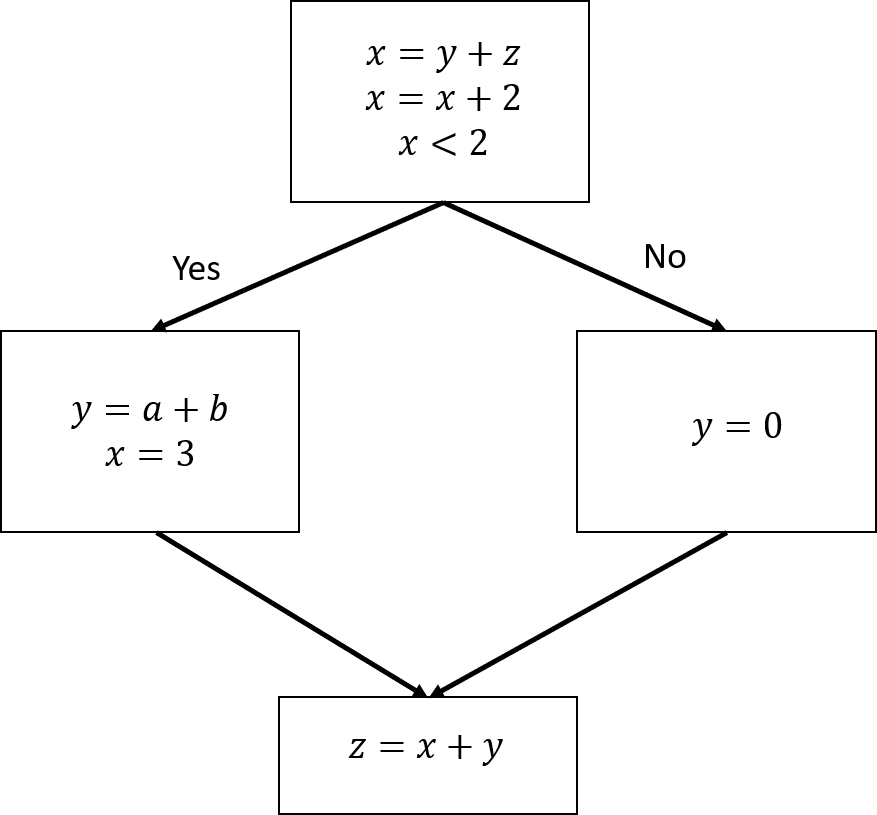
\includegraphics[height=8cm]{images/Example1.png}
\caption{Converting to SSA Example}
\end{figure*}

Consider another example as shown in Figure 1:

In this example, there are 2 variables of interest. $x$ is assigned thrice and $y$ is assigned thrice. On applying the rules of SSA conversion, here is how the code snippet looks like.

The versioning is straightforward for variable $x$. For $y$ in this example, there are two versions reaching at the bottom block from two different paths. The question is how we version the variable $y$ at bottom block. To answer that , we need to understand about basic block
\begin{figure*}
\centering
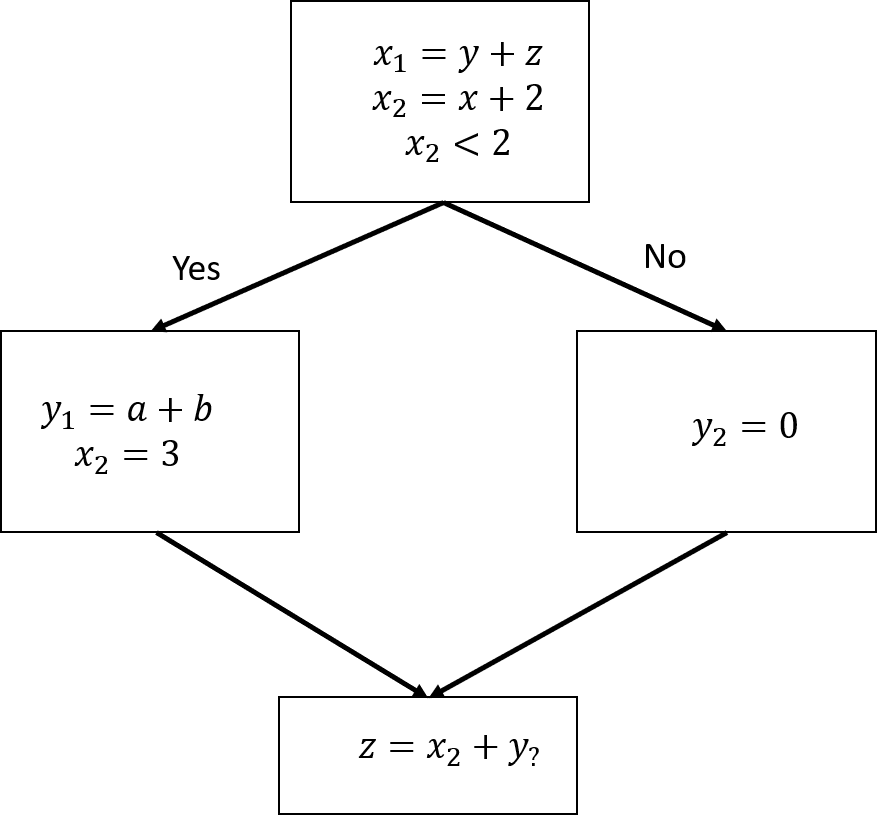
\includegraphics[height=8cm]{images/Example2.png}
\caption{Converting to SSA Example - With Versions}
\end{figure*}

\subsection{Basic Block}: 
A basic block is a maximal set of instructions with 
\begin{itemize}
    \item no labels( except at the first instruction)
    \item no jumps (except in the last instruction)
\end{itemize}

In the example, each rectangle is a basic block. 
Idea:
\begin{itemize}
    \item Cannot jump into a basic block (except at beginning)
    \item cannot jump out of a basic block (except at end)
    \item Single-entry single-exit straight line code segment
\end{itemize}

At the bottom block, there are two version reaching for variable $y$. To represent that we use $\Phi$ node or $\Phi$ function. So the version of y can be represented as a function of $y_1$ and $y_2$ as shown in figure XXX. This is an ordered set.


\begin{figure*}
\centering
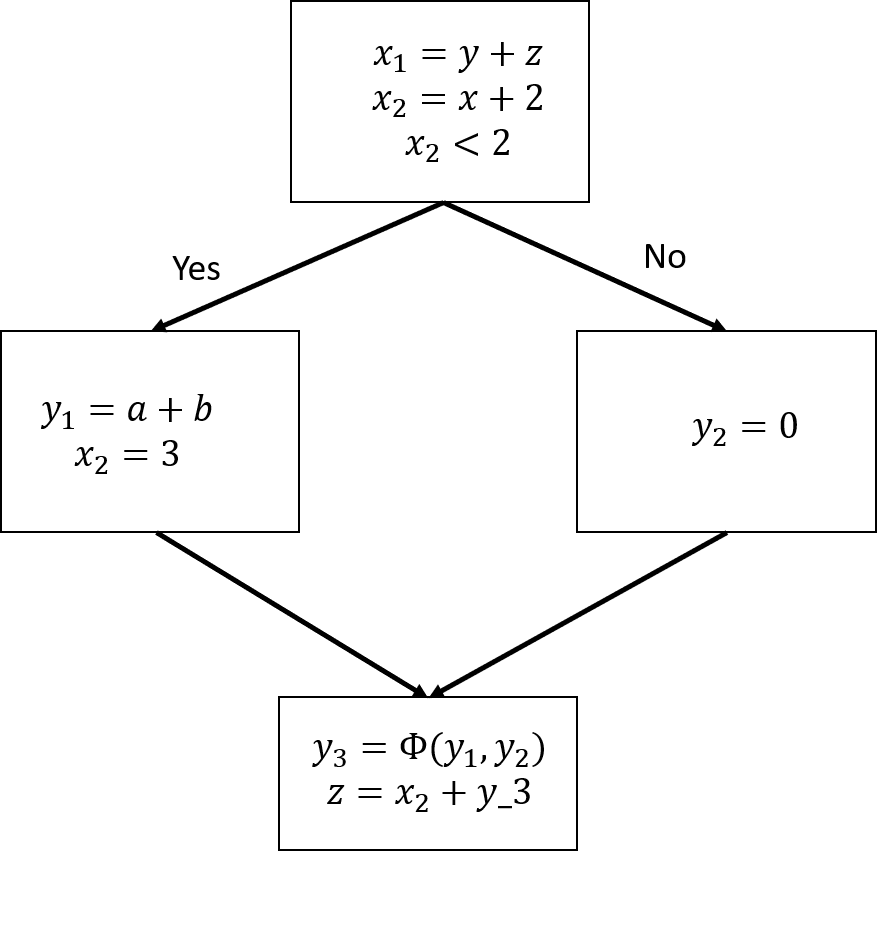
\includegraphics[height=8cm]{images/Example3.png}
\caption{Converting to SSA Example - PHI Nodes}
\end{figure*} 

\subsection{PHI($\Phi$) Nodes}
\begin{itemize}
    \item $\Phi$ function chooses the version depending on the incoming edge.
    \item Present only at the beginning of a basic block. Since this is the only place where there are multiple versions flowing through different incoming edges.
\end{itemize}

